\documentclass[12pt]{article}

% Packages for double-spacing
\usepackage{setspace}
\usepackage{graphicx}
\usepackage{mathbbol}
\doublespacing
\boldmath

\begin{document}

% Title and author information
\title{Graph Neural Network Model}

\maketitle

% Abstract
\begin{abstract}
    A remarkable number of ideas across various domains can be effectively
    depicted as graphs, ranging from social networks and railway maps to
    molecules. Graphs offer an elegant way to abstract these concepts, making
    them a primary tool for representing data. This abstraction not only
    highlights the characteristics of individual data points but also captures
    the relationships between them. However, this versatility poses a challenge
    in the field of machine learning, as desining algorithms that efficiently
    handle such interconnected data has proven to be a challenging task.
\end{abstract}

% Introduction
\section{Introduction}
      We  shall  start  by  giving a brief introduction to out mathematical model. A
    graph  $G$  is  a  pair  $(V,  E)$,  where  $V$  is  the set of vertices, and $E
    \subseteq  V  \times  V$  is  the  set  of edges, representing the relationships
    between  the  vertices.  An  example  of  a  graph would be a railway map, where
    the  vertices  are  the  stations  and  the  edges  are  the railways connecting
    them.  Often  we're  interested  in  giving some attributes to the edges. In the
    case  of  the  railway  map,  we  could  assign the length of the railway to the
    edges,  in  which  case  the graph would be a weighted graph. On the other hand,
    edges   could   be  multidemensional,  in  which  case  the  graph  would  be  a
    hypergraph,  which  is  especially  useful for representing molecules, where the
    vertices are the atoms and the edges are the bonds between them.

     \begin{figure}[h]
         \centering
         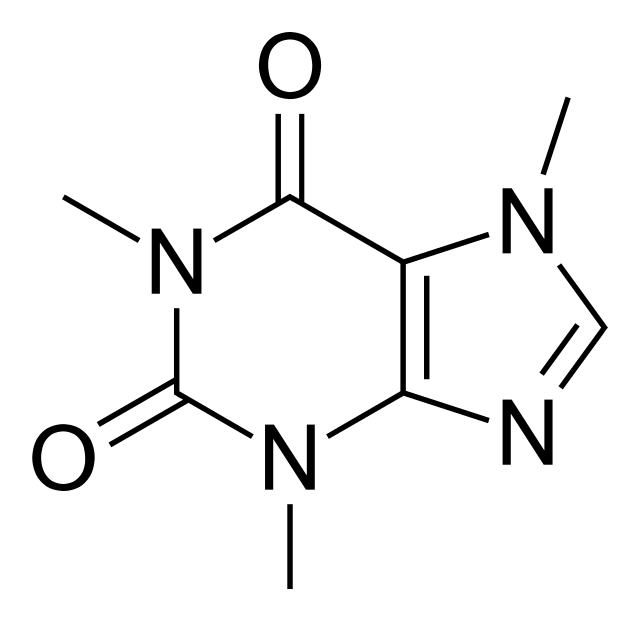
\includegraphics[width=0.4\textwidth]{img/Caffeine_structure.png}
           \caption{A   molecule   of  caffeine,  represented  as  a  graph,  where  the
        vertices are the atoms and the edges are the bonds between them.}
         \label{fig:graph}
     \end{figure}
    
    While providing the definitions, we will stick to unweighted and undirected, i.e.
    simple,  graphs.  The model can be easily extended to other cases.
    For a vertex $v \in V$, the set $N(v) = \{u \in V : (u, v) \in E\}$ is called the
    neighborhood  of  $v$. The  degree  of  a  vertex  $v$  is  $|N(v)|$,  i.e. the
    number  of  vertices  adjacent  to  $v$.
    \\

    For any meaningful application of graphs in data science and machine learning, we
    shall assign labels (real vectors) to the vertices and the edges. They will be represented by
    $l_v \in \mathbb{R}^{l_V}$ and $l_{(v, u)} \in \mathbb{R}^{l_E}$, respectively.

    

% Methodology
\section{The Graph Neural Network Model}
    \indent 
    In this section, we will present the Graph Neural Network model, which is a
    powerful algorithm for learning on graphs, first introduced by Scarselli et al.
    \cite{scarselli2009graph}. 
    \\
    \indent The novelty of the model lies in the fact that it is able to learn the relationships
    between the vertices of a graph, as the representation of each vertex depends on the
    representations of its neighbors.

    More formally, assume we are given a dataset of graphs: \\ $\mathcal{D} = \{(G_i, v_{i, j}, t_{i, j}) | G_i = (V_i, E_i), v_{i, j} \in V_i, t_{i, j} \in \mathbb{R}^m\}$, \\
    where $v_{i, j}$ is the $j$-th vertex of the $i$-th graph, and $t_{i, j}$ is the target label of $v_{i, j}$.
    The objective is to learn a function $\varphi : G \times V \rightarrow \mathbb{R}^m$ such that $\varphi(G_i, v_{i, j}) \approx t_{i, j}$,
    where $G$ and $V$ are the set of all graphs and vertices, respectively, considered in $\mathcal{D}$.
    \\
    \indent The underlying intuitive idea of this algorithm is that in a graph, vertices are representing object, data points, etc.,
    while the edges are representing the relationships between them. Therefore, the representation of a vertex should depend on the
    representations of its neighbors. To mimic this, we will attach a \textbf{\textit{state}} to each vertex, 
    $x_v \in \mathbb{R}^s$, which is encodes information contained in $N(v)$.

% Results
\section{Results}
This is the results section of your article.

% Conclusion
\section{Conclusion}
This is the conclusion section of your article.

% References
\begin{thebibliography}{9}
\bibitem{scarselli2009graph}
Scarselli, F., Gori, M., Tsoi, A. C., Hagenbuchner, M., \& Monfardini, G. (2009). The graph neural network model. IEEE Transactions on Neural Networks, 20(1), 61-80.

\end{thebibliography}

\end{document}




